\documentclass[a4paper, 12pt]{article}

%% Language and font encodings
\usepackage[english]{babel}
\usepackage[utf8x]{inputenc}
\usepackage[T1]{fontenc}

%% Sets page size and margins
\usepackage[a4paper,top=3cm,bottom=3cm,left=3cm,right=3cm,marginparwidth=1.8cm]{geometry}

%% Useful packages
\usepackage{amsmath}
\usepackage{graphicx}
\usepackage[colorinlistoftodos]{todonotes}
\usepackage[colorlinks=true, allcolors=blue]{hyperref}
\setlength{\parindent}{0pt} %首行不縮進
\setlength{\parskip}{8pt} %段落間隔長度
\usepackage{booktabs} %表格
\usepackage{enumerate} %list
\usepackage{amsmath}
\usepackage{algorithm}
\usepackage[noend]{algpseudocode}
\usepackage{subcaption}
\usepackage{listings}
\lstset{
    %backgroundcolor=\color{red!50!green!50!blue!50},
%   rulesepcolor= \color{gray},
    breaklines=true,
    numbers=left,
    numberstyle= \small,
    %keywordstyle= \color{blue},
    commentstyle=\color{gray}
%   frame=shadowbox
    frame=single,
}
\usepackage{hyperref}
\hypersetup{hidelinks,
    colorlinks=true,
    allcolors=black,
    pdfstartview=Fit,
    breaklinks=true}

\title{7CCSMAMF Agent-Based Modelling in Finance\\
Market Manipulation\\
Group Grape}
\author{Yu-Hsun Wang, Pin-Chi Chen, Hsiao-Ching Liu \\ Bo Xu, Xuanming Gu}
\date{} %do not show dates

\begin{document}
\maketitle
\thispagestyle{empty}
\newpage
\setcounter{page}{1}
\section{Introduction}
Financial markets are complex systems that are characterized by the interaction of various agents with different goals, beliefs, and strategies. Understanding how these agents behave influences the market is crucial for policymakers, investors, and traders alike. In recent years, studying the impact of big investors on financial markets has been a big issue. Big investors are institutional investors with a large amount of capital that they can use to influence the market and profit from market trends and fluctuations.\par

This report presents a model that simulates the behavior of various agents in a financial market, including random traders, chartists, and big investors. The model assumes a closed environment and a limit order book (LOB) mechanism. It also incorporates a momentum strategy that uses Moving Average Convergence Divergence(MACD) as a key technical indicator for implementing trading decisions.\par

The focus of this report is to examine the manipulation effect of big investors on the market. Specifically, we investigate how big investors use their enormous capital and complex strategies to generate upward momentum and profit from the market. We also examine the impact of big investors on the volatility of the market and their interaction with other agents, such as chartists and random traders.



\section{Methodology}
    \subsection{Model assumptions}

        The model has several assumptions, which include:
        \begin{enumerate}
            \item \emph{Closed environment}: The model assumes that the market is closed, which means all the agents are allocated with a given amount of money and asset (finite) and then start trading,no money is created during the whole process.
            \item \emph{Three types of agents}: The model includes three types of agents: random traders, chartists and big investors.
            \item \emph{Fixed order quantity}: We assume that every investor sends an equal number of orders (each order's quantity is fixed to 1) for the same asset. The investor must wait until its execution or expiration to send another order.
            \item \emph{No regulatory measures or transaction taxes}
            
        \end{enumerate}
        
    \subsection{Market mechanism}
        Our model follows the mechanism of a \textbf{limit order book (LOB)}, a popular market mechanism used in financial markets. In a LOB, each trader has a belief in the value of stocks, randomly set at the beginning. Time is split into ticks, and traders use a pre-determined strategy to put orders on the market in each tick.\par
        
        Sell orders are matched with buy orders at the stated price or higher, and the two parties exchange stocks and cash. If a sell order isn't fully executed, it goes into the unmatched list. Buy orders go through the same process, but with an opposite bias to match lower prices. The market price and other information are calculated and given to traders in the next tick.

    
    \subsection{Market participants and Strategies}
        Assume there are three types of traders in the market, \textbf{random agents}, \textbf{chartists} and \textbf{big investors}.
        \subsubsection{Random Agents}
            \textbf{Random agents} buy, sell and hold an asset with an equal probability. Their actions mainly add liquidity to the market and allow other traders to apply their strategies.
        
            The strategy uses the formulas $P_b(t+1)=P(t)\cdot N(\mu_b,\sigma_t)$ and $P_s(t+1)=P(t)\cdot N(\mu_s,\sigma_t)$ to compute buy and sell order prices, respectively. In these formulas, $P(t)$ represents the current stock price at time $t$, while $N(\mu_b,\sigma_t)$ and $N(\mu_s,\sigma_t)$ are random numbers drawn from a Gaussian distribution. By setting the mean value of $\mu_b$ to 1.01 and $\mu_s$ to 0.99, and adjusting the volatility factor with $\sigma_t$ calculated based on the asset's price volatility in the previous 10 time steps, the trading environment is stimulated, and the volatility of the system is increased. This approach has been observed in the work of Raberto et al. (2001) [1], where a similar volatility factor is used in price formation.

        \subsubsection{Chartists}
            \textbf{Chartists} are technical analysts who identify patterns of the stock market to predict stock price movements by identifying patterns. When there are more chartists in the market, the stock tends to have higher volatility.

            In this model, \emph{Chartists} utilize the \textbf{Moving Average Convergence Divergence (MACD)} as their primary technical analysis tool, recognizing its effectiveness in identifying the underlying trend in asset prices and providing valuable insights into market momentum and direction. The MACD is a powerful indicator, designed to assist traders in making informed decisions by analyzing the relationship between two moving averages and generating signals that can help them stay ahead of market movements. Section 2.4 provides details on how this indicator is used in the strategy.
        
        
        
        \subsubsection{Big Investors}

            
            \textbf{Big investors} have enormous capital and use more complex strategies than other market traders. They aim to profit from market trends and fluctuations by buying at lower prices and selling at higher prices.

            \emph{The big investor} follows a strategy of buying low and selling high, utilizing \textbf{MACD} but with a different duration compared to chartists. When the Momentum Strategy signals a buying position, the investor will start to purchase a large proportion of market sell orders (75-95\%) until 50\% of the strategy duration has elapsed. A brief pause follows, during which there only exist chartists and random agents trading in the market. As it reaches the last 25\% and prices stii remain in a high position, the \emph{big investor} gradually sells the orders they hold in a small portion of all the buy orders in the market (20-35\%), until all orders have been sold. This strategy allows the investor to purchase at a lower price, generate upward momentum, and sell later for a profit.
            

    \subsection{Momentum Strategy}
        In this model, we are utilizing the \textbf{Moving Average Convergence Divergence (MACD)} strategy.

        The MACD indicator is calculated by subtracting the 26-day EMA from the 12-day EMA. Therefore, the MACD uses EMAs as its basis for calculation.
        
        \subsubsection{EMA}
            According to Kirkpatrick II and Dahlquist (2010) [2], the exponential moving average (EMA) at time t is defined as:
    
            $$\text{EMA}(t) = (\text{P}(t) * \text{W}) + \text{EMA}(t-1) * (1 - \text{W})$$
            where:
    
            \begin{itemize}
                \item $\text{P}(t)$ is the asset’s price at time $t$
                \item $\text{W}$ is the weighting multiplier, it is computed as: $\text{W}= 2 ÷ (N_{EMA} + 1)$
                \item $N_{EMA}$ is the number of days in moving average
                \item $\text{EMA}(t-1)$ is the exponential moving average at time $t-1$
            \end{itemize}
    
        \subsubsection{MACD}

            The formula for the MACD is:

            $$ \text{MACD Line} = \text{12-day EMA} - \text{26-day EMA} $$
            
            $$ \text{Signal Line} = \text{9-day EMA} \text{ of the MACD Line} $$
            
            
            When the MACD line crosses above the signal line, it generates a \textbf{buying signal}, indicating a potential upward price trend. On the contrary, it generates a \textbf{selling signal}, indicating a potential downward price trend.

        
    \subsection{Model parameters}

        \subsubsection{Market Size}
            The market comprises of 201 investors, which can be classified into three groups: 180 \emph{random agents}, 20 \emph{chartists} and 1 \emph{big investor}.
            
        
        \subsubsection{Initial Wealth of investors}
            \emph{Random agents} and \emph{chartists} are defined to hold asset of 80 shares of and money of \$1000. \emph{The big investor} holds a variable amount of wealth, determined by a slider, which can be adjusted to see how it affects the result of the manipulation. \emph{The big-investor's wealth} is represented by a multiple of the initial wealth of the other investors. For example, if the slider is set to 100,000, then \emph{the big investor} would start with 8,000,000 shares and \$100,000,000 of cash, which is 100,000 times the initial wealth of the other investors.

        \subsubsection{Strategy-related Parameters}
            
            The duration of big investor's strategy is parameterized to last for 100 ticks, allowing us to observe its impact on the market and asset pricing.

        \subsubsection{Order Expiration}    
            When an order reaches its lifespan limit, it will be deleted in the market by the system. The orders in the market expire every 15 ticks, with each tick representing one time step (t+1).

        \subsubsection{Depletion Behavior}
            When an investor's stock inventory drops to zero, they have a 25\% chance of submitting a buy order to acquire more shares, while the remaining 75\% of the time they hold their current position. Likewise, when an investor runs out of available funds, they have a 25\% chance of submitting a sell order to liquidate their current holdings, with a 75\% chance of holding their position. 

        \subsubsection{Pseudo Code}
        \begin{algorithm}[H]
        \caption{Market Simulation with Limit Order Book}
        \label{alg:market_simulation}
        \begin{algorithmic}[1]
        \State Initialize the simulation environment with the LOB
        \While{simulation not complete}
        \State Expire old orders in the LOB
        \State Random traders place new buy/sell orders in the LOB
        \State The big investor and the chartists place buy/sell orders in the LOB using the MACD indicator
        \State Match and execute orders in the LOB based on price-time priority
        \State Update investor wealth and stock price based on executed trades
        \State Calculate indicators such as traders' wealth, standard deviation, and trading volume
        \State Update simulation time
        \EndWhile
        \State Output final results, including stock price and agent wealth distribution
        \end{algorithmic}
        \end{algorithm}
        

\section{Results}
We conducted three distinct scenarios to analyze the stock market. The first scenario (S1) involved only random agents trading. The second scenario (S2) included chartists alongside random agents. Finally, the third scenario (S3) incorporated the big investor.\par

\begin{table}[h!]
\centering
\caption{Summary of Scenarios}
\label{tab:scenarios}
\begin{tabular}{@{}ccc@{}}
\toprule
\textbf{Scenario} & \textbf{Agents} & \textbf{Description} \\ \midrule
S1 & Random & Only random agents \\
S2 & Random and Chartists & Chartists added \\
S3 & Random, Chartists, and Big Investor & Big investor added \\ \bottomrule
\end{tabular}
\end{table}

In section 3.1, the diagrams represented random agents trading exclusively (S1).

Moving on to section 3.2, we compared the scenarios of S2 and S3 to observe the impact of the big investor on stock prices and the sigma of the stock price. This allowed us to identify the substantial influence of the big investor on the market.

In section 3.3, we analyzed the sigma distribution across the three different scenarios to determine the volatility range of each scenario.

Finally, in section 3.4, we discussed the return rate of the three types of agents during scenario 3, where the big investor was included. This analysis enabled us to evaluate the performance of each type of agent in the presence of the big investor.\par

\subsection{Scenario 1: Only Random Agents}

\begin{figure}[h!]
    \centering
    \begin{minipage}{0.45\textwidth}
        \centering
        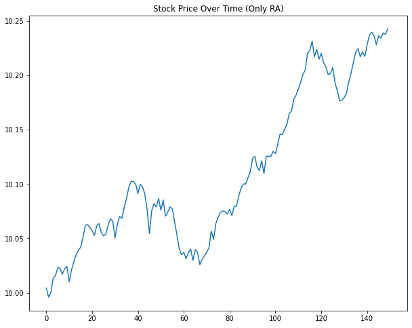
\includegraphics[width=\textwidth]{price_s1.png}
        \label{fig:my_label1}
    \end{minipage}
    \hfill
    \begin{minipage}{0.45\textwidth}
        \centering
        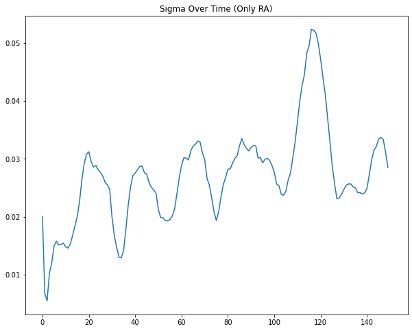
\includegraphics[width=\textwidth]{sigma_s1.png}
        \label{fig:my_label2}
    \end{minipage}
\end{figure} 

\textbf{Figure 1, 2. The stock price and sigma generated by random agents in 150 ticks.}\par

The first scenario aimed to create market liquidity over a 150-tick period by having only random agents send buy or sell orders at random intervals. As a result, the stock price underwent significant fluctuations as the random agents' actions had a direct impact on the market.\par

To better understand the characteristics of the scenarios involving chartists and the big investor, we would conduct a comparison analysis with the first scenario. This comparison analysis allowed us to identify the key features of scenarios S2 and S3, and to evaluate the impact of adding chartists and the big investor to the market. By comparing the outcomes of these scenarios, we gained insight into the behavior of different types of investors and their effects on the stock price and volatility levels.\par

\vspace{\baselineskip}

\subsection{Single Pump-and-Dump Analysis}

\begin{figure}[h]
    \centering
    \begin{minipage}{0.5\textwidth}
        \centering
        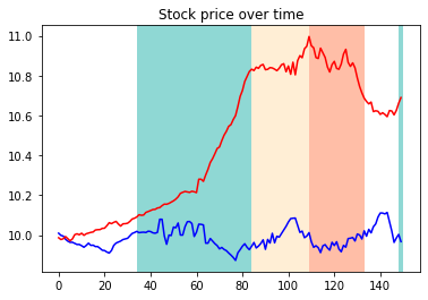
\includegraphics[width=\textwidth]{price_s3.png}
        \label{fig:my_label3}
    \end{minipage}
    \hfill
    \begin{minipage}{0.45\textwidth}
        \centering
        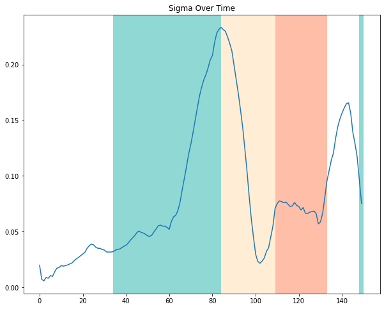
\includegraphics[width=\textwidth]{sigma_s3.png}
        \label{fig:my_label4}
    \end{minipage}
\end{figure} 

\vspace{\baselineskip}

\textbf{Figure 3. Compared the stock price over 150 ticks across two different scenarios: S2 (blue line) and S3 (red line).}\par
It demonstrated how the stock price changed significantly after adding a big investor. The big investor influenced this market's stock price, leading to market manipulation. The red line also climbed considerably in the green zone due to the big investor purchases at that time. This was followed by a modest fluctuation in the yellow part, which varied from 85 to approximately 110, and then experienced a moderate downward trend in the orange section as the result of the big investor's stock sale.\par

\vspace{\baselineskip}

\textbf{Figure 4. The market's overall sigma over S3}\par
Sigma enabled us to identify the pump-and-dump behavior of the big investor simultaneously. During the pump (green zone), the volatility would upsurge. It would plummet to almost zero when the big investor's strategy reached the static stage and then went up to a certain level when the dump occurred.\par

\subsection{Sigma Analysis}

The big investor significantly increased market volatility (sigma) compared to the other two scenarios, which affected the magnitude of stock price movements. We can easily compare the three scenarios with the histograms on the right side.\par

\begin{figure}[h!]
    \centering
    \begin{subfigure}{0.5\textwidth}
        \centering
        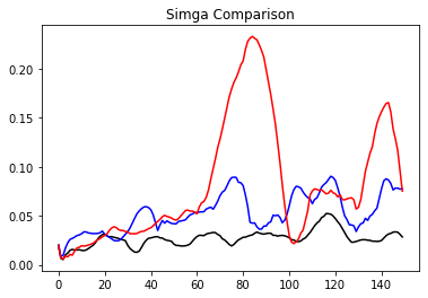
\includegraphics[width=\textwidth]{sigma_s3-2.png}
        \label{fig:my_label5}
    \end{subfigure}
    \hfill
    \begin{subfigure}{0.45\textwidth}
        \centering
        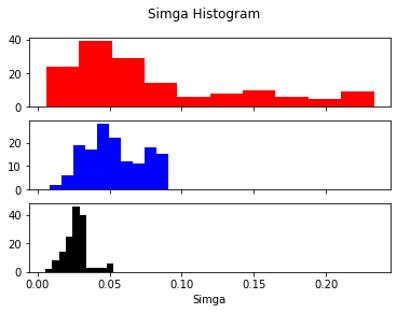
\includegraphics[width=\textwidth]{sigma_h.png}
        \label{fig:my_label6}
    \end{subfigure}
\end{figure} 


\textbf{Figure 5, 6. Sigma comparison via line graph and three histograms
The red line contained three categories of investors: random agents, chartists, and a big investor in the 150 ticks doing a single pump and dump. The blue line included random agents and chartists. The black line represented only random agents.}\par


Based on the histogram depicted on the right, it is evident that the sigma of S1, which involves only random agents, is concentrated between 0 and 0.05. However, when chartists are incorporated, the volatility range widens and falls within 0 and 0.09. Subsequently, with the inclusion of the big investor, the sigma distribution takes a right-tailed shape, where the proportion of extreme values increases significantly, and the overall range is between 0 and 0.24. Hence, it is apparent that the presence of the big investor has a substantial impact on the sigma. Thus, it can be inferred that the addition of the big investor plays a crucial role in determining the volatility of the market.\par

\subsection{Return Analysis}
\vspace{\baselineskip}
In order to create a more robust and comprehensive model, we increased the number of ticks from 150 to 2000, thereby including several pumps and dumps in our analysis. This enabled us to observe the market over a more extended period and obtain a more accurate representation of the behavior of different investors.\par

\begin{table}[h]
\centering
\caption{Return Rate of Different Types of Investors in S3 over 2000 ticks}
\label{tab:returnrate}
\begin{tabular}{@{}lc@{}}
\toprule
\textbf{Investor Type} & \textbf{Return Rate} \\ \midrule
Random Agents & -29.05\% \\
Chartists & 109.03\% \\
The Big Investor & 157.06\% \\ \bottomrule
\end{tabular}
\end{table}

Upon analysis of the resulting data, we observed that the big investor outperformed the other investors by a significant margin. The big investor's return rate of 157.06\% was notably higher than that of the chartists, who had a return rate of 109.03\%. Additionally, the return rate of the random agents was negative at -29.05\%, indicating that they performed poorly in this scenario.\par

Our findings suggest that the big investor had a considerable advantage over the other investors, possibly due to their greater financial resources and market influence. The big investor's significant return rate may have been a result of their ability to influence the market through their trading activity, leading to an increased demand for the stock and driving up prices. This, in turn, may have allowed the big investor to sell their shares at a higher price, resulting in a substantial profit.\par

\subsection{Sensitivity Analysis}
 In this section, we changed three parameters(buy\_ratio, sell\_ratio and b\_multiplier) and found that changing of these parameters had no effect on the normal behavior of model. We can conclude that the model is robust to these parameters.

\section{Conclusion}

\subsection{Potential Mitigation Strategies}

To conclude, market manipulation can cause significant damage to the financial market and individual investors. In order to prevent market manipulation, we come up with multiple strategies in two aspects. First, enhanced market surveillance is fundamental to avoid the occurrence of manipulation. To achieve that, we mainly implement advanced data analytics and artificial intelligence techniques to monitor market activities in real time. Additionally, detecting unusual trading patterns is also an efficient way to help us identify potential pump-and-dump schemes early. 

Secondly, market regulators should figure out ways to Increase transparency in financial markets, especially in emerging areas. Encouraging greater transparency in financial markets can be realized by mandating timely and accurate disclosure of relevant information and promoting the use of secure and transparent platforms for conducting market transactions.

\subsection{Future work}

Despite we have built the model and identified some key characteristics by running the model, there are many potential ideas which need to be discarded. 

Future research can be done to explore the dynamics of market manipulation by looking into how variations of strategies of big investors can have an effect on the market, and then evaluate the efficacy of these strategies. Moreover, new tactics and techniques that can be used by market manipulators to stay ahead of regulatory efforts need to be identified. The last important issue for future work is how manipulation responds to regulation.

\section{Bibliography}
    \begin{thebibliography}{1}
    \bibitem{key-1}Raberto, M., Cincotti, S., Focardi, S. M., \& Marchesi, M. (2001). Agent-based simulation of a financial market. Physica A: Statistical Mechanics and Its Applications, 299(1–2), 319–327. https://doi.org/10.1016/S0378-4371(01)00312-0


    \bibitem{key-2}Kirkpatrick II, C. D. and Dahlquist, J. A. (2010) “Technical analysis: the complete resource for financial market technicians”. FT press.
    
    \end{thebibliography}
\clearpage
\section*{Appendix A}
\subsection*{click the link to see our python code}
\href{github}{https://github.com/AuroraLiu3230/Market-Manipulation-Model}


\clearpage
\section*{Appendix B}
\begin{figure}[h]
    \centering
    \begin{subfigure}{0.3\textwidth}
        \centering
        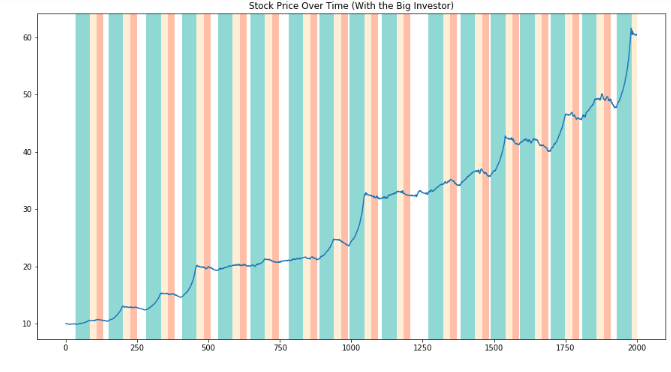
\includegraphics[height=80pt,width=\textwidth]{p1.png}
        \label{fig:my_label7}
    \end{subfigure}
    \hfill
    \begin{subfigure}{0.3\textwidth}
        \centering
        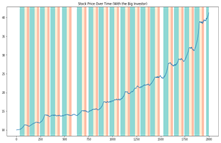
\includegraphics[height=80pt,width=\textwidth]{p2.png}
        \label{fig:my_label8}
    \end{subfigure}
    \hfill
    \begin{subfigure}{0.3\textwidth}
        \centering
        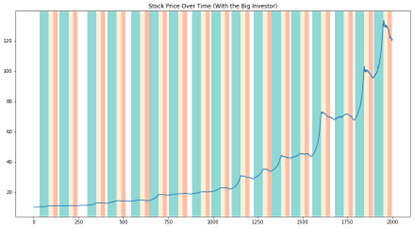
\includegraphics[height=80pt,width=\textwidth]{p3.png}
        \label{fig:my_label9}
    \end{subfigure}
\end{figure} 


\textbf{Figure 7, 8 , 9. Different output of stock price over time when buy ratio is 0.75 , 0.8 , 0.85 in the premise that sell ratio remains the same.}\par

\begin{figure}[h]
    \centering
    \begin{subfigure}{0.45\textwidth}
        \centering
        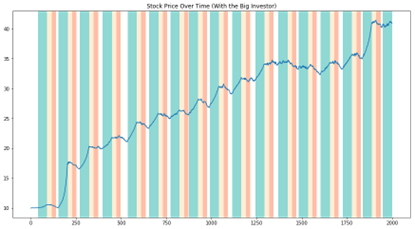
\includegraphics[height=80pt,width=\textwidth]{p4.png}
        \label{fig:my_label10}
    \end{subfigure}
    \hfill
    \begin{subfigure}{0.45\textwidth}
        \centering
        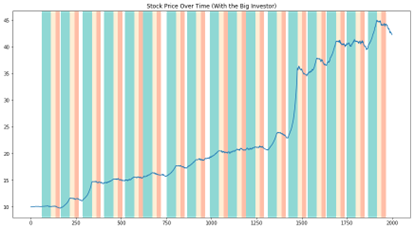
\includegraphics[height=80pt,width=\textwidth]{p5.png}
        \label{fig:my_label11}
    \end{subfigure}
\end{figure}

\textbf{Figure 10, 11. Different output of stock price over time when sell ratio is 0.25 , 0.3 in the premise that buy ratio remains the same.}\par

\begin{figure}[h]
    \centering
    \begin{subfigure}{0.45\textwidth}
        \centering
        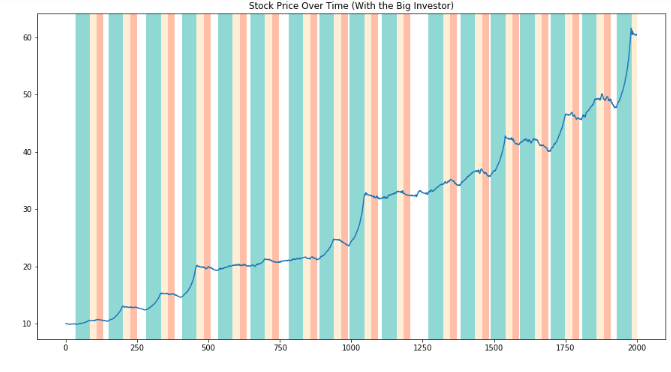
\includegraphics[height=80pt,width=\textwidth]{p1.png}
        \label{fig:my_label12}
    \end{subfigure}
    \hfill
    \begin{subfigure}{0.45\textwidth}
        \centering
        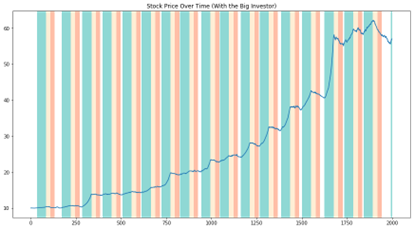
\includegraphics[height=80pt,width=\textwidth]{p6.png}
        \label{fig:my_label13}
    \end{subfigure}
\end{figure}

\textbf{Figure 12, 13. Different output of stock price over time when big investor multiplier is 100000 , 1000000 in the premise that buy ratio and sell ratio remain the same.}\par
\end{document}